\documentclass[10pt,twocolumn]{article}

\usepackage[letterpaper,margin=0.68in,columnsep=0.24in,includeheadfoot,headheight=18pt]{geometry}
\usepackage{amsmath,amsthm}
\usepackage{newtxtext,newtxmath}
\usepackage[scaled=0.92]{helvet}
\usepackage{booktabs}
\usepackage{graphicx}
\usepackage{caption}
\usepackage{microtype}
\usepackage[table]{xcolor}
\usepackage{titlesec}
\usepackage{fancyhdr}

\definecolor{ink}{HTML}{16212B}
\definecolor{navy}{HTML}{17324D}
\definecolor{accent}{HTML}{0B7A75}
\definecolor{muted}{HTML}{667085}
\definecolor{wash}{HTML}{F1F6F6}
\usepackage[colorlinks=true,linkcolor=accent,citecolor=accent,urlcolor=accent]{hyperref}

\setlength{\parindent}{1em}
\setlength{\parskip}{0pt}
\setlength{\textfloatsep}{7pt plus 2pt minus 2pt}
\setlength{\floatsep}{6pt plus 2pt minus 2pt}
\setlength{\intextsep}{6pt plus 2pt minus 2pt}
\renewcommand{\arraystretch}{1.05}
\color{ink}
\captionsetup{font=small,labelfont={bf,sf,color=navy},skip=4pt}

\titleformat{\section}
  {\sffamily\large\bfseries\color{navy}}
  {\color{accent}\thesection}{0.55em}{}[\vspace{0.18em}\color{accent!35}\titlerule]
\titlespacing*{\section}{0pt}{1.25ex plus .2ex minus .1ex}{1.1ex}
\titleformat{\paragraph}[runin]
  {\sffamily\bfseries\color{navy}}{}{0pt}{}[.]
\titlespacing*{\paragraph}{0pt}{0.7ex}{0.45em}

\pagestyle{fancy}
\fancyhf{}
\fancyhead[L]{\sffamily\scriptsize\color{muted} BLINDED INVERSE TAKEOFF}
\fancyfoot[R]{\sffamily\scriptsize\color{muted}\thepage}
\renewcommand{\headrulewidth}{0.25pt}
\renewcommand{\headrule}{\hbox to\headwidth{\color{accent!45}\leaders\hrule height \headrulewidth\hfill}}

\newtheoremstyle{cleanprop}
  {0.5ex}{0.5ex}{\itshape}{} {\sffamily\bfseries\color{navy}}{.}{0.45em}{}
\theoremstyle{cleanprop}
\newtheorem{proposition}{Proposition}
\newcommand{\NN}{\mathbb{N}}

\begin{document}
\raggedbottom
\twocolumn[{
\begin{@twocolumnfalse}
\vspace*{-1.75em}
\noindent{\sffamily\bfseries\fontsize{23}{26}\selectfont\color{navy}
Blinded Inverse Takeoff}\par
\vspace{0.38em}
\noindent{\sffamily\fontsize{14}{17}\selectfont\color{muted}
Finite-horizon limits in recovering recursive redundancy}\par
\vspace{0.65em}
\noindent{\sffamily\small\color{ink} Jonathan R. Landers\hfill July 2026}\par
\vspace{0.5em}
\noindent\color{accent}\rule{\textwidth}{1.2pt}\par
\vspace{0.65em}
\noindent\colorbox{wash}{%
  \parbox{\dimexpr\textwidth-2\fboxsep\relax}{%
  \small\color{ink}\textbf{Abstract.}\enspace
Memoization collapses repeated calls in a recursion tree into shared states.
The velocity takeoff profile records how quickly that redundant work appears
as input size grows. This note studies the inverse question: can a finite,
noisy takeoff trace reveal the recurrence that produced it? We give an exact
finite-horizon obstruction. For every observation length there are distinct
aperiodic nonnegative-integer recurrences with the same terminal tree speed,
the same total branching, the same polynomial memoized-state growth, and an
identical observed takeoff prefix. We then report two blinded AWS sweeps
containing 1.16 million hidden schemas and 32.67 million recovery trials. A
generic matrix-pencil baseline succeeds on many visible short-lag recurrences
but fails sharply on the constructed hidden-lag family. Under noise, accurate
forecasting often survives after modal identification has collapsed. The
result is both a negative theorem and a practical warning: predicting a
recursive response is not the same as identifying its mechanism.
  }}
\vspace{0.9em}
\end{@twocolumnfalse}
}]

\section{Why invert a takeoff curve?}

A naive recursive program exposes a tree of calls. Equal labels can appear
many times; memoization identifies them and leaves a directed acyclic graph
(DAG) of distinct subproblems. Let $N_n$ be the number of calls in the naive
tree on input size $n$, and let $M_n$ be the number of distinct reachable
labels. The logarithmic overlap is
\[
S_n=\log\frac{N_n}{M_n},
\]
with one-step velocity
\[
v_n=S_{n+1}-S_n=u_n-w_n,
\]
where
\[
u_n=\log N_{n+1}-\log N_n,\qquad
w_n=\log M_{n+1}-\log M_n.
\]
If $N_n$ grows exponentially with speed $\alpha>0$ while $M_n$ is
polynomial, then $u_n\to\alpha$, $w_n\to0$, and $v_n\to\alpha$. That terminal
number says how fast redundancy eventually accumulates, but not how it gets
there. Two recurrences can have the same cruising speed while one accelerates
immediately and the other rings for a very long time.

The normalized takeoff profile and its causal difference are
\[
F_n=\frac{u_n}{\alpha},\qquad
\kappa_n=F_n-F_{n-1},\quad F_{-1}=0.
\]
Thus $F_n\to1$, and $\kappa$ records the response shape: delay, monotone
settling, alternating correction, or damped ringing. Forward analysis starts
from a recurrence and predicts $F$. Inverse takeoff starts from an observed
prefix of $F$ and asks what can be recovered.

The analogy is system identification, but the object is unusual. The
``plant'' is the redundant response of a recursion tree before memoization
quotients equal states. Classical Prony and matrix-pencil methods can estimate
damped exponential modes from samples \cite{prony,hua,plonka}. What is new is
the constrained source class and the distinction between response modes and
literal recursive branches.

\section{Finite-lag response and its modes}

Consider the finite-lag schema
\begin{equation}
N_n=1+\sum_{j\in J}a_jN_{n-j},\qquad N_m=1\ \text{for }m\le0,
\label{eq:recurrence}
\end{equation}
where $J\subset\{1,2,\ldots\}$ is finite and
$a_j\in\mathbb{Z}_{>0}$. Define
\[
Q(z)=1-\sum_{j\in J}a_jz^j.
\]
When $\gcd(J)=1$ and $\sum_j a_j>1$, $Q$ has a unique smallest-modulus
positive root $\rho\in(0,1)$, and the terminal speed is
$\alpha=-\log\rho$. Non-dominant singularities $\zeta$ contribute normalized
correction modes
\[
\theta=\frac{\rho}{\zeta}.
\]
The affine $+1$ in \eqref{eq:recurrence} also contributes the singularity
$z=1$. The largest active $|\theta|<1$ controls the eventual settling rate,
while a complex leading mode produces ringing.

For a common terminal speed $\alpha=\log2$, the root is $\rho=1/2$ and the
coefficient constraint becomes
\begin{equation}
\sum_j a_j2^{-j}=1.
\label{eq:fixedspeed}
\end{equation}
This dyadic identity is useful experimentally: it generates many structurally
different recurrences while holding the first-order asymptotic invariant
exactly fixed.

An observed tail is modeled approximately as
\begin{equation}
Y_n:=F_n-1\approx\sum_{r=1}^{m}c_r\theta_r^n.
\label{eq:modal}
\end{equation}
The approximation matters. Even when $N_n$ has a finite exponential
expansion, the logarithmic ratio defining $F_n$ introduces higher-order mode
products. A low-rank spectral fit is therefore a tail model, not an algebraic
identity for every finite prefix.

Figure~\ref{fig:atlas} gives a visual vocabulary for the inverse problem. The
top row is the takeoff profile; the bottom row is its causal difference, the
kernel actually carrying the transient shape. The same terminal level can be
approached smoothly, by sign alternation, through damped oscillation, or in
widely separated echoes.

\begin{figure*}[p]
\centering
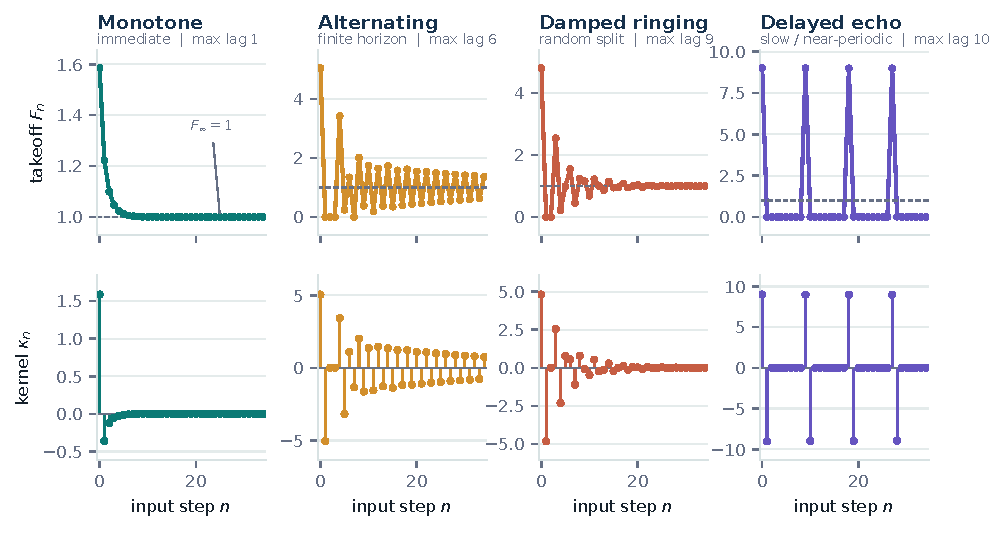
\includegraphics[width=0.94\textwidth]{figures/kernel_atlas.pdf}
\caption{\textbf{A kernel atlas from representative experimental schemas.}
All four recurrences have terminal speed $\alpha=\log2$ and hence
$F_n\to1$, but their finite responses are plainly different. The dashed line
marks the common terminal level. The lower row shows
$\kappa_n=F_n-F_{n-1}$: a short relaxation, alternating correction, damped
ringing, and a near-periodic echo train. Different vertical scales are used so
that each transient remains legible.}
\label{fig:atlas}
\end{figure*}

\section{An exact finite-horizon obstruction}

The central difficulty is more basic than numerical noise: the recursive
signal may not yet have returned from its hidden lag.

\begin{proposition}[Fixed-invariant finite-horizon nonidentifiability]
Fix an integer observation length $T$. There exist distinct aperiodic
finite-lag schemas satisfying \eqref{eq:fixedspeed}, having the same total
branch count and $M_n=O(n)$, whose takeoff profiles agree exactly on
$F_0,\ldots,F_{T-1}$.
\end{proposition}

\begin{proof}
Choose $L\ge T$ and an integer
$1\le t<2^{L+1}/3$. Set
\[
a_L=t,\quad
a_{L+1}=2^{L+1}-3t,\quad
a_{L+2}=2t.
\]
All three coefficients are positive. Their total is
$A=2^{L+1}$, independent of $t$, and
\[
4a_L+2a_{L+1}+a_{L+2}=2^{L+2},
\]
which is \eqref{eq:fixedspeed} after division by $2^{L+2}$. Hence every member
has $\alpha=\log2$. The consecutive support
$\{L,L+1,L+2\}$ is aperiodic, and its reachable labels lie in a
one-dimensional interval, so $M_n=O(n)$.

For $1\le n\le L$, every referenced boundary value in
\eqref{eq:recurrence} equals one. Therefore
\[
N_1=\cdots=N_L=1+A
\]
for every $t$. It follows that $F_0,\ldots,F_{L-1}$ are identical. At the next
step,
\[
N_{L+1}=1+A+tA,
\]
so different $t$ values separate. They also define distinct polynomials
$Q_t$; because each has constant term one, their full root multisets cannot
all coincide. Thus no estimator receiving only the common prefix can recover
the coefficient vector correctly for every member.
\end{proof}

Intuitively, this is like listening for an echo before sound has reached the
reflecting wall. Unlimited estimator sophistication cannot recover information
that is absent from the observation window. The proposition concerns distinct
combined recurrences, not merely different stories that split the same
coefficients into latent channels. Figure~\ref{fig:collision} shows the
construction directly: different hidden branch allocations have the same
fixed-speed invariant and exactly the same visible prefix, then emit different
echoes when the longest lag begins to return.

\begin{figure*}[p]
\centering
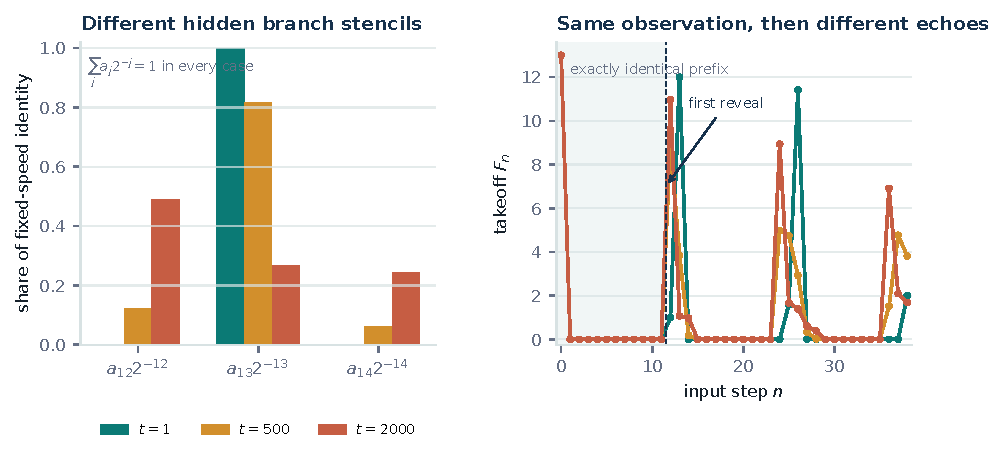
\includegraphics[width=0.94\textwidth]{figures/hidden_lag_collision.pdf}
\caption{\textbf{Exact finite-horizon blindness at $L=12$.}
Left: three distinct coefficient stencils, plotted by their contribution
$a_j2^{-j}$ to the fixed-speed identity. Right: their takeoff profiles coincide
exactly on $F_0,\ldots,F_{11}$ (shaded) and first separate at $F_{12}$. Later
pulse trains retain visibly different recursive signatures. This collision is
algebraic, not a consequence of noise or an unsuccessful optimizer.}
\label{fig:collision}
\end{figure*}

\section{The blinded experiment}

The study used five fixed-speed families: immediate binary recursion; the
near-periodic slow family
$a_L=2^L-1$, $a_{L+1}=2$; the proposition's finite-horizon family; a two-scale
family with one local and one delayed channel; and random dyadic refinements
that replace one branch at lag $j$ by two branches at lag $j+1$. Every such
refinement preserves \eqref{eq:fixedspeed}.

For each hidden schema we computed an exact integer call-count sequence and
formed $F_n$. The estimator received only
\[
\widetilde Y_n=Y_n+\sigma
\max\{\operatorname{RMS}(Y),10^{-12}\}\,\xi_n,
\qquad \xi_n\sim\mathcal N(0,1),
\]
not the coefficients or true roots. We tested windows beginning at the origin
and immediately after the maximum lag. Relative noise levels were
$0,10^{-8},10^{-5},10^{-3}$.

The baseline formed Hankel matrices
\[
(H_0)_{ij}=\widetilde Y_{i+j},\qquad
(H_1)_{ij}=\widetilde Y_{i+j+1},
\]
selected an order from one through six by held-out prediction, and recovered
poles from a truncated-SVD matrix pencil. It then forecast 24 unseen samples.
We scored the leading-pole radius, qualitative class (monotone, alternating,
or ringing), and holdout normalized RMSE. ``Forecast success'' means NRMSE
below $0.1$. Ground truth was used only after fitting.

Two independent seeded sweeps were run. Table~\ref{tab:runs} reports launcher
wall time, which slightly overstates billable instance time. At the verified
rate of \$1.428/hour, estimated compute was \$0.782 total. Both instances
terminated and all temporary cloud resources were removed.

\begin{table}[t]
\centering
\caption{Completed AWS runs.}
\label{tab:runs}
\small
\begin{tabular}{lrrr}
\toprule
Run & Schemas & Trials & Time \\
\midrule
Broad baseline & 575,440 & 13,810,560 & 18.6 min \\
Horizon sweep & 589,302 & 18,857,664 & 14.2 min \\
\midrule
Total & 1,164,742 & 32,668,224 & 32.8 min \\
\bottomrule
\end{tabular}
\end{table}

The broad run used lengths $24,48,96$ and lags through 18. The horizon sweep
used lengths $8,16,32,64$ and lags through 32, permitting explicit bins in
$T/L$. Each schema contributed every window, regime, and noise condition; the
schema generator itself was stochastic rather than an exhaustive uniform
census.

\begin{figure*}[!t]
\centering
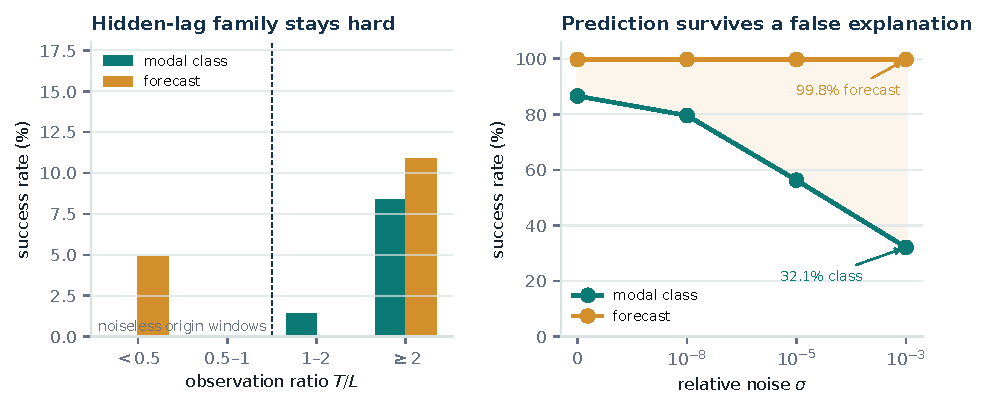
\includegraphics[width=0.94\textwidth]{figures/aws_recovery_results.pdf}
\caption{\textbf{Recovery phase diagrams from the completed AWS sweeps.}
Left: on the constructed finite-horizon family, noiseless origin-window
recovery is absent below the hidden lag and remains weak after it becomes
visible. Right: on 144,863 post-lag random-split schemas with a 96-sample
window, modal classification degrades sharply with relative noise while
24-step forecast success remains 99.8\%. Bars and curves are computed directly
from the saved run summaries.}
\label{fig:aws-results}
\end{figure*}

\section{Results}

Figure~\ref{fig:aws-results} summarizes the two most important empirical
boundaries: information arriving after the hidden lag, and prediction
remaining reliable after modal identification degrades.

\paragraph{Sub-lag observations are blind.}
Table~\ref{tab:horizon} isolates noiseless finite-horizon traces beginning at
the origin. Modal-class accuracy was zero throughout $T/L<1$. This empirical
zero is consistent with the proposition, although the theorem itself proves
coefficient nonidentifiability rather than a particular classifier's error.
There is no rapid recovery immediately after the lag: the generic six-mode
baseline remained poor even for $T/L\ge2$. These schemas can have degree 34
and crowded near-periodic modes, so the post-lag failure is an empirical
limitation of the baseline, not a second impossibility theorem.

\begin{table}[t]
\centering
\caption{Noiseless finite-horizon family, origin windows.}
\label{tab:horizon}
\small
\begin{tabular}{lrrr}
\toprule
$T/L$ & Trials & Class acc. & Forecast succ. \\
\midrule
$<0.5$ & 101,309 & 0.0\% & 4.9\% \\
$[0.5,1)$ & 132,303 & 0.0\% & 0.0\% \\
$[1,2)$ & 147,761 & 1.4\% & 0.0\% \\
$\ge2$ & 209,671 & 8.4\% & 10.9\% \\
\bottomrule
\end{tabular}
\end{table}

\paragraph{The estimator is not universally ineffective.}
Random dyadic-split recurrences were much easier once observations began after
the largest lag. In the noiseless broad run, class accuracy was 78.3\%, 88.9\%,
and 86.6\% for windows 24, 48, and 96; forecast success was 95.6\%, 99.5\%, and
99.8\%. The corresponding sampled median leading-radius errors were 0.0024,
0.0007, and 0.0005. Thus the hard-family failure is structurally selective.

\paragraph{Prediction can survive a false explanation.}
For post-lag random-split traces of length 96, raising relative noise from zero
to $10^{-3}$ reduced modal-class accuracy from 86.6\% to 32.1\% and increased
sampled median radius error from 0.0005 to 0.4453. Forecast success nevertheless
remained 99.8\%. A finite-window predictor can therefore extrapolate accurately
while assigning the wrong modal geometry. This is the most practically
important empirical warning: predictive fit, modal identification, and source
identification are three different evidentiary levels.

\section{What the experiment establishes}

The exact contribution is modest but sharp. Without a lag bound, finite-prefix
source recovery is impossible even after terminal speed, total branching, DAG
growth class, and aperiodicity are fixed. The experiment then shows where a
standard spectral tool works and where it does not. Massive replication makes
the family contrast stable; it does not turn the classical matrix-pencil
algorithm into a novel method.

Several limitations matter. The schemas are synthetic and one-dimensional;
real program traces may contain input-dependent branching and measurement
artifacts. The modal baseline is capped at order six, while the hardest
recurrences have much larger degree. Root calculations for high-degree,
near-periodic polynomials are themselves conditioned problems. The logarithmic
takeoff profile is only asymptotically a finite exponential sum, and very small
late corrections approach floating-point resolution. Finally, millions of
trials do not remove bias from the chosen schema distribution.

The next positive result should exploit information the baseline ignores:
\[
a_j\in\mathbb Z_{\ge0},\qquad
\sum_j a_j2^{-j}=1,
\]
together with a declared lag bound and sparsity. A constraint-aware decoder can
enumerate or optimize over feasible dyadic recurrences, forward-simulate their
takeoff curves, and compare them on held-out samples. The academically useful
test is whether those constraints shift the recovery boundary as a function of
$T/L$, noise, pole separation, and modal radius. Real recursive traces should
then test whether the recovered equivalence classes remain stable outside the
synthetic model.

\section{Conclusion}

Recursive redundancy casts a modal shadow, but a short shadow does not uniquely
reveal the object that cast it. Before the longest lag returns, distinct
fixed-speed recurrences can be exactly observationally identical. Afterward,
generic modal recovery may work well on ordinary short-lag families yet remain
fragile on nearly periodic ones. Most strikingly, excellent forecasts can
coexist with incorrect modes. Inverse takeoff should therefore report what the
data support in order: response prediction first, modal structure second, and
literal recursive mechanism only under explicit identifying constraints.

\newpage
\begin{thebibliography}{9}
\small

\bibitem{prony}
G. de Prony.
Essai exp\'erimental et analytique.
\emph{Journal de l'\'Ecole Polytechnique}, 1:24--76, 1795.

\bibitem{hua}
Y. Hua and T. K. Sarkar.
Matrix pencil method for estimating parameters of exponentially
damped/undamped sinusoids in noise.
\emph{IEEE Transactions on Acoustics, Speech, and Signal Processing},
38(5):814--824, 1990.

\bibitem{plonka}
I. Keller and G. Plonka.
Modifications of Prony's method for the recovery and sparse approximation of
generalized exponential sums.
\emph{Springer Proceedings in Mathematics \& Statistics}, 2020.

\bibitem{flajolet}
P. Flajolet and R. Sedgewick.
\emph{Analytic Combinatorics}.
Cambridge University Press, 2009.

\bibitem{michie}
D. Michie.
``Memo'' functions and machine learning.
\emph{Nature}, 218:19--22, 1968.

\end{thebibliography}

\end{document}
